\documentclass[12pt,a4paper]{article}
\usepackage[utf8]{inputenc}
\usepackage{graphicx}
\usepackage{amsmath}
\usepackage{mathtools}
\usepackage[utf8]{inputenc}
\usepackage{float} 
\usepackage{subfigure}
\usepackage{ragged2e}
\usepackage{blindtext}
\usepackage{graphicx}
\usepackage[nodoi,nonurl]{apacite} % APA 6 Citation style

\begin{document}
\begin{titlepage}
	\centering
	
\includegraphics[width=0.5\textwidth]{UZH LOGO.png}\par\vspace{1cm}
	%{\scshape\LARGE Digital Tools for Finance \par}
	{\scshape\LARGE Digital Tools for Finance \par}
	\vspace{1cm}
	{\scshape\Large Final Project\par}
	\vspace{1.5cm}
	{\huge\bfseries Beta and Stock Returns\par}
	{\large\bfseries A Portfolio Analysis\par}
	\vspace{2cm}
	\leftline
	{\Large\itshape Kevin Hardegger     12-758-785\par}
	\vspace{1cm}
	\leftline
	{\Large\itshape Kun Zhang   20-746-892\par}
	\vspace{1cm}
	\leftline
	{\Large\itshape Ruixuan Zhou    15-727-019\par}
	\vspace{1cm}
	\leftline
	{\Large\itshape Ziyun Ni    19-764-182\par}
	\vspace{1cm}
	\vfill\large
	supervised by\par
	Dr.~Igor \textsc{Pozdeev}
	\vfill

% Bottom of the page
    \vspace{1cm}
	{\large Submission Date: \today\par}
\end{titlepage}

\renewcommand*\contentsname{Table of Contents}
\tableofcontents
\addtocontents{toc}{~\hfill\textbf{Page}\par}
\vspace{1cm}
\listoffigures
\vspace{1cm}
\listoftables

\newpage
\setcounter{page}{1}


\section{Introduction}
The Capital Asset Pricing Model (CAPM) introduces a theory of asset valuation. Nowadays, nearly six decades later, it is still the most prevalent used model to explain the relationship between risk and expected return of a certain asset. The foundation for this model was established by \citeA{Markowitz_1952} and further developed by \citeA{Sharpe_1964}, \citeA{Lintner_1965}, and \citeA{Mossin_1966} into what we know today as CAPM. In 1952, Markowitz introduced the concept of mean-variance efficient portfolios, which means that investors choose portfolios that maximize expected returns at a given level of variance and minimize the variance at a given level of expected return. In addition to Markowitz, Tobin (1958) introduced the separation theorem, where he introduced the concept of borrowing and lending in portfolio construction. Not long after, Sharpe and Lintner introduced the assumption that investors share a common probability distribution function, which contrasts with the assumptions of Markowitz, who stated that each investor has his own probability distribution. They also introduced the CAPM. The CAPM states that the return on each asset is explained by its market beta, and only the market beta is sufficient to explain the expected return.

In this short paper, we will test the CAPM empirically by evaluating beta-sorted portfolio. In chapter 2 we will shortly introduced the CAMP and the definition of beta. In Chapter 3, we create 5 portfolios based on the magnitude of security's beta and consider them to examine the validity of CAMP. Subsequently, we provides the results of time-series in order to investigate the relation between beta and expected returns. Finally, Chapter 4 presents the conclusion based on our empirical findings.


\section{Beta as risk measure}
\begin{justify}
According to the CAPM of \citeA{Sharpe_1964}, \citeA{Lintner_1965}, and \citeA{Mossin_1966} the expected return of any stock is equal to the return on the riskless asset plus the market beta of this stock plus the market risk premium. Expressed mathematically, the CAPM is given by
\begin{align}
    E[R_{i,t}] = R_{f,t}+\beta_{i}(E[R_{m,t}-R_{f,t}])
\end{align}
where the security’s beta is given by

\begin{align}
    \beta_{i} = \frac{Cov(R_{i,t},R_{m,t})}{Var(R_{m,t})} 
\end{align}

Here, $R_{i,t}$, $R_{m,t}$, and $R_{f,t}$ denotes the return of stock i, the market portfolio, and the risk-free asset in period t. The difference between the expected return of the market portfolio and the risk-free rate $E[R_{m,t}-R_{f,t}]$ is defined as the market risk premium. $\beta_{i}$ is the beta of stock i and can be computed as the covariance between the return of stock i and the market return divided by the variance of the return of the market return in period t.
 
The fundamental prediction of the CAPM theory is that there is a positive relation between market beta and expected stock returns, and the slope defining this relation represents the market risk premium. In addition, the CAPM predicts that variation in the expected returns on any stocks should be  driven by variation in the betas of the stock only \cite{Bali2016}. Thus, we would expect to find a positive cross-sectional relation between beta and future excess return.
\end{justify}

\section{Empirical research}
\subsection{Evaluating beta-sorted portfolios}
First, we created time series for both datasets, daily betas and daily prices of all stocks that belonged to the SMI. Second, we used daily prices to estimate the daily returns for each stock. Then, for each period of the time series, we ranked the stocks included in the SMI based on their betas in the previous period and divided them into 5 portfolios based on the quintiles 20\%, 40\%, 60\% and 80\%. Portfolios 1 contains stocks with lowest beta and Portfolio 5 contains stocks with highest beta. Subsequently, we continued this process until the last period of the time series. Finally, for each portfolio we calculated the average daily return and the average standard deviation of the daily returns. The table below summarizes the results:
~\\

\makeatletter\def\@captype{table}\makeatother
\centering
\resizebox{1\textwidth}{!}{%
\begin{tabular}{|l|c|c|c|c|c|}
\hline
\multicolumn{1}{|l|}{} & P1      & P2      & P3      & P4      & P5      \\ \hline
Mean daily return      & 0.027\% & 0.035\% & 0.041\% & 0.058\% & 0.039\% \\ \hline
Mean standard deviation           & 0.958\% & 1.268\% & 1.455\% & 1.620\% & 1.972\% \\ \hline
\end{tabular}%
}
\caption{Mean daily returns \& mean standard deviation of each beta-sorted portfolio}
\label{tab:my-table}

~\\
\begin{justify}
From above, we can clearly see that the mean standard deviation is low if a portfolio contains stocks with low beta and is high if a portfolio contains the stocks high beta. The magnitudes of the mean daily returns of portfolios 1 to 4 is consistent with the magnitudes of their mean standard deviation. The higher the average standard deviation respective the volatility, the higher the average daily return. One exception is the portfolio 5. It has the highest volatility but surprisingly not the highest mean return, which contradicts the Mean-Variance theory.

To ensure that the daily beta values of each portfolio are always correctly ranked within the observation period, we also draw a line chart showing the average daily beta value for each portfolio. From the figure below, one can observe that the daily beta the portfolio 5 always lies above the daily beta of portfolio 4 at any given time,and so forth.

\begin{figure}[H]
\centering
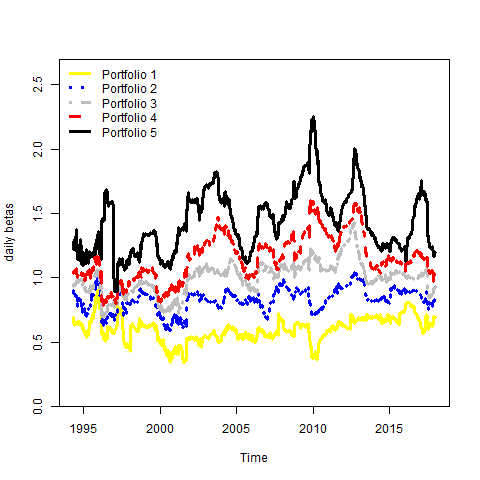
\includegraphics[width=1\textwidth,height=0.8\textwidth]{daily betas}
\caption{Development of daily betas}
\label{fig:Development of daily betas}
\end{figure}

We then calculated cumulative returns for each portfolio and we then plotted them. The plot of the development of each portfolio’s cumulative returns is shown below
\begin{figure}[H]
\centering
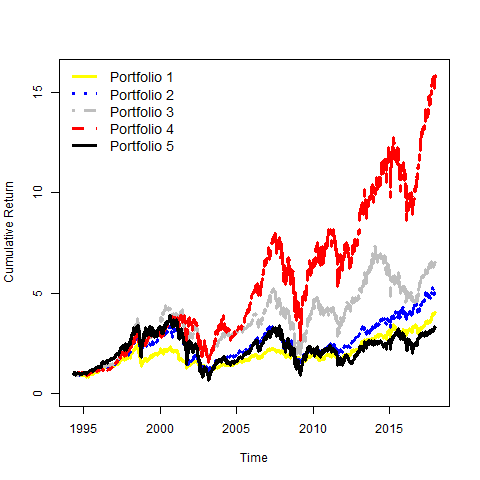
\includegraphics[width=1\textwidth,height=0.8\textwidth]{Cumulative Returns}
\caption{Development of Cumulative Returns of Portfolios}
\label{fig:Development of Cumulative Returns of Portfolios}
\end{figure}




From the above chart, we can clearly see that the cumulative return of portfolio 4 is the highest, although the beta of the stocks contained in portfolio 4 are only the second highest. The magnitudes of the cumulative returns of portfolios 1 to 4 is also consistent with the magnitudes of the betas of stocks contained in each portfolio. But surprisingly, although Portfolio 5 contains stocks with the highest beta, his returns are the lowest, which contradicts the CAPM theory that predicts a positive relation between beta and expected returns.
The risk of a stock can be measured by its standard deviation. However, it can be reduced by diversification effect respective by holding other stocks in a portfolio. This means that the right way to measure the risk of a stock is not by its standard deviation but rather by its covariance with the market portfolio. Thus, the CAPM beta should be a more appropriate risk measure.  However, our empirical result above fails to produce supporting evidence,  since portfolio 5, according to the CAPM theory, should have the highest cumulative return among portfolios sorted by beta.

\subsection{Comparision with other benchmark assets}
In this section, we introduce two benchmark asset to compare the returns of beta-sorted portfolios. One of them is the SMI Exchange Traded Fund (ETF) from which the portfolios are built from. SMI ETF is our proxy for the market portfolio and should therefore have a beta of one. The other one is the 1 Year Swiss Government Bond in order to simulate the return of riskless assets with a beta of zero. 

After creating time-series of both benchmark asset, we now compare the cumulative returns between each beta-based portfolio, SMI ETF, as well as the 1Year Swiss Government Bonds. The line chart below indicates that portfolio 5 provides the lowest cumulative return for all equity based portfolios. The cumulative return even sinks below that of the 1YR Swiss Government Bond twice; in the year 2003 and 2009. This heavily contradicts the CAPM, as the highest beta portfolio should earn the highest risk premium. All other beta sorted portfolio seem to outperform both the SMI and the 1YR Swiss Gov Bond.    
\begin{figure}[H]
\centering
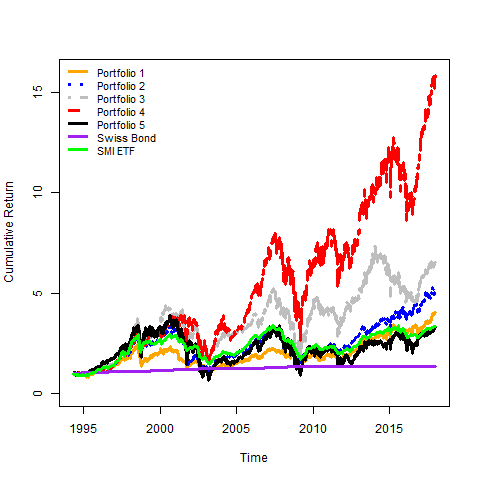
\includegraphics[width=1\textwidth,height=0.8\textwidth]{Cumulative Returns with SMI&SGB.png}
\caption{Development of Cumulative Returns of Portfolios and benchmarks}
\label{fig:Development of Cumulative Returns of Portfolios and benchmarks}
\end{figure}


\section{Conclusion}
We see that the highest beta does not promise the highest return. On the contrary, the portfolio containing the stocks with the highest beta values performed even poorer than the benchmark the SMI. The portfolio containing the fourth quintile of highest beta values, delivered the highest return by a large margin instead. Furthermore, we see that portfolio 3 with its average beta value of 1 has outperformed the SMI as well. As the SMI is weighted according to market capitalization and contain roughly 20 stocks, it may not be as diversified as needed. Thus, its beta value may differ that from a true market portfolio and could indicate that the SMI fails to represent a market portfolio in compliance with the CAPM. Another caveat is that we didn't include transaction costs. Nevertheless, the results are startling. As a next step, larger stock markets from other countries should be analysed to see if these findings can be reinforced.



\newpage

\bibliographystyle{apacite}
\bibliography{References.bib}
\end{justify}
\end{document}